\chapter{Đặt vấn đề}
\label{chap1}

Sự phát triển mạnh mẽ của lĩnh vực công nghệ thông tin đã góp phần giúp cuộc sống
của con người ngày trở nên dễ dàng và tiện lợi. Tận dụng các thành tựu của khoa học
công nghệ, nhiều trang thương mại điện tử ra đời và ngày càng lớn mạnh với sự tham
gia của đông đảo người dùng tiêu biểu như: Facebook, Youtube, Netflix, Amazon,
Twitter, v.v.. Thông qua các trang thương mại điện tử này, quá trình tiếp thị của những
nhà cung cấp dịch vụ và sản phẩm trở nên đơn giản và dễ dàng thông qua các hình thức
quảng cáo. Tuy nhiên, số lượng sản phẩm và dịch vụ ngày càng nhiều, người dùng cần
phải tốn nhiều thời gian hơn trong quá lựa chọn. Đây là tình trạng quá tải thông tin, gây
ra sự bất tiện và khó khăn trong quá trình trích lọc thông tin của người dùng. Ngoài ra,
người dùng cũng phải đối mặt với nghịch lý rằng có rất nhiều sản phẩm để lựa chọn
nhưng lại không chọn ra được một sản phẩm thích hợp.

Với hiện trạng nêu trên, hệ tư vấn ngày càng đóng vai trò quan trọng trong sự phát
triển của thường mại điện tử. Theo Wikipedia, hệ tư vấn là các kỹ thuật được sử dụng
nhằm mục đích dự đoán điểm đánh giá mà người dùng có thể dành cho một sản phẩm.
Các điểm đánh giá dự đoán này là cơ sở để thực hiện tư vấn sản phẩm phù hợp cho
người dùng. Hiện nay, các hệ thống lớn cung cấp sản phẩm, dịch vụ đều phát triển hệ tư
vấn của riêng mình, tiêu biểu như: hệ tư vấn phim của Netflix, hệ tư vấn âm nhạc của
Pandora, hệ tư vấn sách của Amazon [4]. Theo [4], khi sử dụng hệ tư vấn, nhà cung cấp
sản phẩm và dịch vụ có thể nhận lại rất nhiều lợi ích trong đó có: tăng doanh thu bán
hàng và sự hài lòng của khách hàng. Tuy nhiên, để có thể tư vấn chính xác, hệ tư vấn
cần được cung cấp các dữ liệu liên quan tới sở thích và nhu cầu của người dùng. Sở
thích và nhu cầu của người dùng thể hiện qua: lịch sử tìm kiếm, lịch sử mua hàng, đánh
giá sản phẩm, v.v.. Những dữ liệu này đóng vai trò quyết định tới kết quả tư vấn của hệ
thống.

Trong mạng xã hội, mỗi người dùng có một không gian riêng và có thể kết nối với
nhau thông qua danh sách bạn bè. Trong không gian này, người dùng có quyền làm
những gì họ muốn trong phạm vi hỗ trợ của nền tảng mạng xã hội, chẳng hạn như: chia
sẻ một bộ phim, bình luận về một bài viết, kết bạn và theo dõi. Những hành động trên
được gọi chung là hành vi của người dùng trên mạng xã hội. Các hành vi của người
dùng trên mạng xã hội phản ánh một phần sở thích, tính cách và quan điểm của họ đối
với những sự kiện xảy ra trên mạng xã hội. Điều này có ảnh hưởng không nhỏ tới những
người trong danh sách bạn bè của họ.
\begin{figure}[htbp]
    \centering
    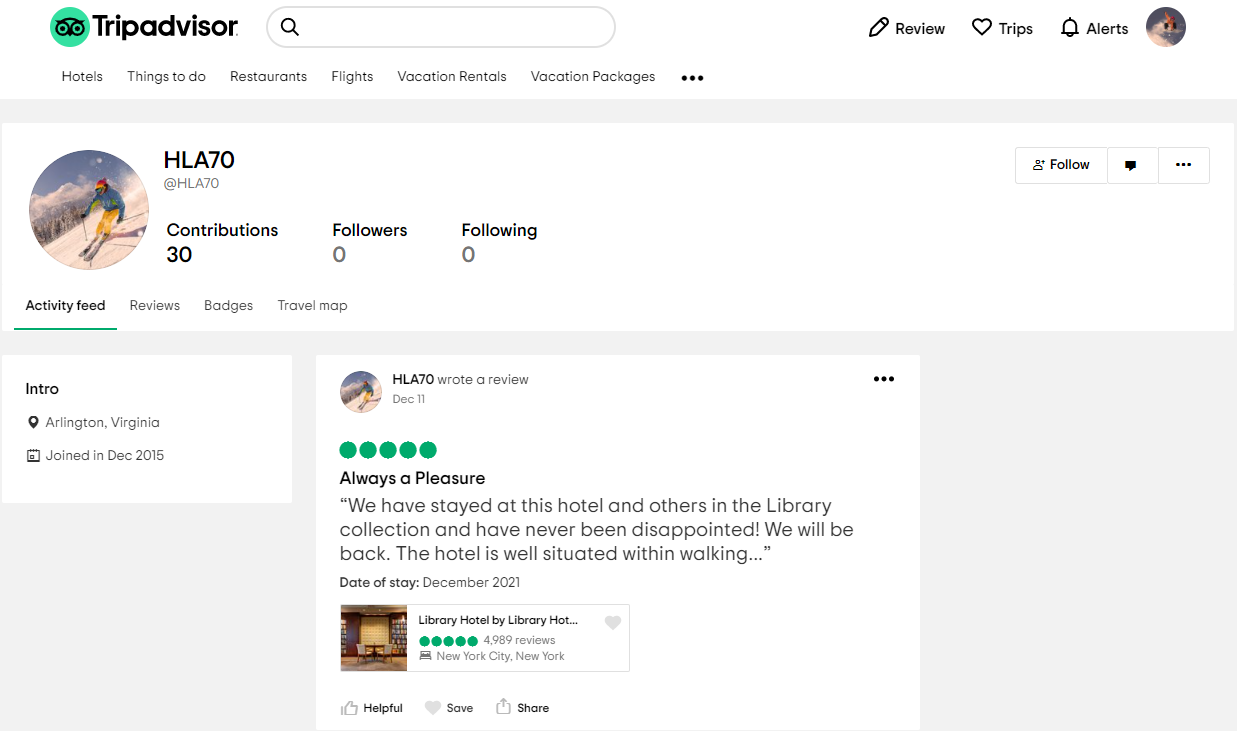
\includegraphics[width=1\linewidth]{imgs/chapter_3/trip-advisor.png}
    \caption{Trang cá nhân của một người dùng trên mạng xã hội Tripadvisor}
    \label{trip-advisor}
\end{figure}
Hình \ref{trip-advisor} mô tả trang cá nhân của một người dùng trên mạng xã hội Tripadvisor.
Tripadvisor là một trang chuyên cung cấp thông tin về những địa điểm du lịch: nhà hàng,
khách sạn, danh lam thắng cảnh. Những người dùng trên nền tảng này để lại đánh giá
cho những địa điểm mà họ đã trải nghiệm. Những đánh giá này ảnh hưởng tới quyết
định trải nghiệm du lịch của những người dùng khác. Càng có nhiều người theo dõi thì
mức độ ảnh hưởng của người dùng càng lớn, thể hiện thông qua: số lượng người theo dõi (Followers), tương tác của bài đánh giá (Helpful, Save, Share). Đăng bài đánh giá,
theo dõi, tương tác là những hành vi chính trên mạng xã hội này. Với một bài đánh giá, phần đánh giá điểm và bình luận là 2 phần thể hiện rõ nhất
quan điểm của người dùng. Vì vậy, trong phần tiếp theo, đồ án sẽ tập trung trình bày về
hành vi đánh giá và hành vi bình luận của người dùng trên mạng xã hội.

Cần viết lại cho mượt

Tuy nhiên, hệ khuyến nghị cũng có những điểm yếu cần khắc phục. Theo [3], hệ tư vấn lọc cộng tác là kỹ thuật được sử dụng phổ biến hiện nay nhưng vẫn còn phải đối mặt với những vấn đề điền hình như: khởi đầu lạnh, thưa thớt dữ liệu và khả năng mở rộng. Đầu tiên, vấn đề thưa thớt dữ liệu, một trong những vấn đề chính của hệ tư vấn và ảnh hưởng rất nhiều đến chất lượng của hệ thống. Thông thường, dữ liệu để thực hiện tư vấn của hệ thống được biểu diễn dưới dạng ma trận người dùng-sản phẩm, giá trị của các ô trong ma trận là điểm đánh giá người dùng dành cho sản phẩm đó. Tuy nhiên, do thói quen lười đánh giá của người dùng khiến mật độ các giá trị được điền của ma trận
trở nên thưa thớt. Sự thưa thớt này càng ngày càng tăng lên khi hệ thống phát triển, số
lượng người dùng và sản phẩm tăng lên. Đây vẫn là một vấn đề cần phải được nghiên
cứu thêm. Tiếp theo, vấn đề khởi đầu lạnh xảy ra khi gặp 1 trong 3 tình huống: người dùng
mới, sản phẩm mới và hệ thống mới. Trong những tình huống này, người dùng, sản
phẩm hay hệ thống chưa có dữ liệu để thực hiện khai thác, dự đoán thói quen, nhu cầu
của người dùng. Vì vậy hệ thống rất khó để thực hiện tư vấn. Cuối cùng, khả năng mở rộng là thuộc tính của hệ thống cho thấy khả năng xử lý
lượng thông tin ngày càng tăng một cách hiệu quả. Với sự bùng nổ dữ liệu, đây là một
thách thức lớn đối với các hệ thống khi nhu cầu xử lý thông tin liên tục tăng. Trong lọc
cộng tác, các phép tính phát triển theo cấp số nhân và tốn kém tài nguyên, đôi khi dẫn
đến kết quả không chính xác.